\chapter{Исследовательская часть}

В данном разделе будут приведены примеры работы программа, а также проведен сравнительный анализ реализаций алгоритмов при различных ситуациях на основе полученных данных.

\section{Технические характеристики}

Технические характеристики устройства, на котором выполнялись замеры времени представлены далее:

\begin{itemize}
	\item операционная система Windows 11 Pro Версия 22H2 (22621.674) \cite{wind};
	\item память 16 ГБ;
	\item процессор 11th Gen Intel(R) Core(TM) i5-11400 2.59 ГГц \cite{proc}.
\end{itemize}

При тестировании компьютер был включен в сеть электропитания. Во время замеров процессорного времени устройство было нагружено только встроенными приложениями окружения, а также системой тестирования.

\section{Демонстрация работы программы}

На рисунке \ref{img:res} представлен результат работы программы. На экран выводятся результаты заемров времени для разных размеров матриц и разных видов алгоритмов матричного умножения в мс.
\newpage
%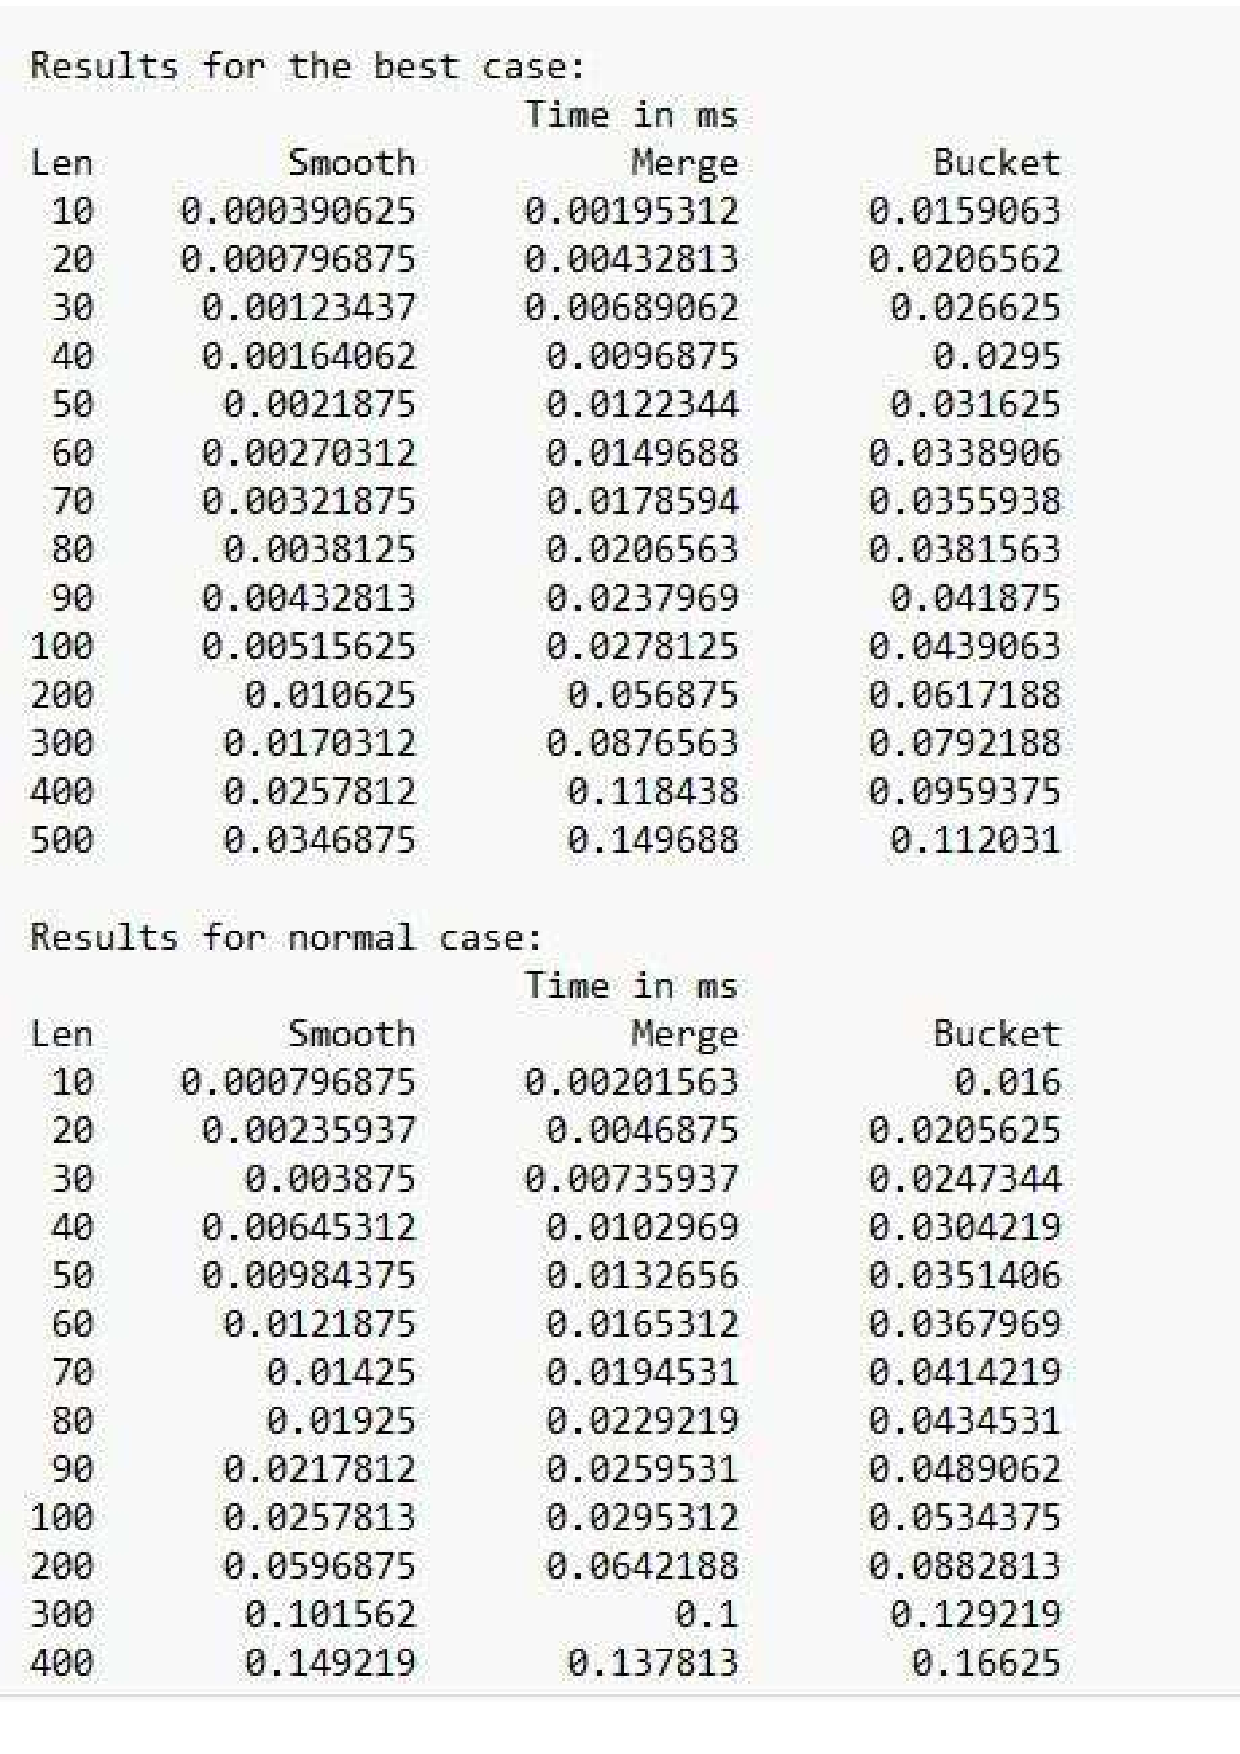
\includepdf[pages=-]{src/screen.pdf}
\begin{center}
	\centering{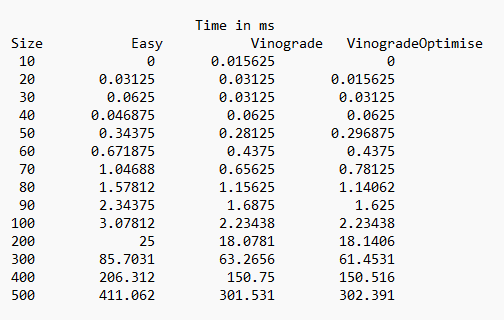
\includegraphics[trim=0 0 0cm 0cm bb=0 0 504 320]{src/screen}}
	\captionof{figure}{Пример работы программы}
	\label{img:res}
\end{center}

\section{Время выполнения реализаций алгоритмов}

Как было сказано выше, используется функция замера процессорного времени GetProcessTimes(...) из библиотеки Windows.h. Функция возвращает пользовательское процессорное временя типа float.

Использовать функцию приходится дважды, затем из конечного времени нужно вычесть начальное, чтобы получить результат.

\textbf{Входные данные:} размер матрицы от 10 до 500, элементы матрицы -- целые числа от 0 до 200.

Результаты замеров времени работы реализаций алгоритмов матричного умножения на различных входных данных (в мс) приведены в таблицах \ref{tbl:best}.


\begin{center}
	\begin{threeparttable}
		\caption{Процессорное время работы реализаций алгоритмов для четной размерности}
		\label{tbl:best}
		\begin{tabular}{|c|c|c|c|}
			\hline
			Размер & Классический &  Винограда &  Оптимизированный\\
			\hline
			10 & 0  &  0.015625 &0  \\ 
			\hline
			20 &0.03125  &      0.03125 &      0.015625\\ 
			\hline
			30 &  0.0625        &0.03125  &      0.03125 \\ 
			\hline
			40 &  0.046875     &    0.0625 &        0.0625  \\ 
			\hline
			50 & 0.34375      &  0.28125    &   0.296875  \\ 
			\hline
			60 & 0.671875    &     0.4375    &     0.4375 \\ 
			\hline
			70 &  1.04688   &     0.65625     &   0.78125 \\ 
			\hline
			80 & 1.57812   &     1.15625       & 1.14062 \\ 
			\hline
			90 & 2.34375  &       1.6875        &  1.625 \\ 
			\hline
			100 & 3.07812&        2.23438        &2.23438 \\ 
			\hline
			200 & 25 &       18.0781      &  18.1406\\ 
			\hline
			300 &  85.7031    &    63.2656 &       61.4531 \\ 
			\hline
			400 &  206.312   &      150.75  &      150.516  \\ 
			\hline
			500 &  411.062  &      301.531   &     302.391  \\ 
			\hline
		\end{tabular}
		
	\end{threeparttable}
\newpage
\begin{threeparttable}
	\caption{Процессорное время работы реализаций алгоритмов для нечетной размерности}
	\label{tbl:best}
	\begin{tabular}{|c|c|c|c|}
		\hline
		Размер & Классический &  Оптимизированный Винограда  &  Винограда\\
		\hline
		11 &  0.015625 &      0.015625      & 0.015625 \\ 
		\hline
		21 &  0.0625    &   0.046875       &0.046875  \\ 
		\hline
		31 & 0.15625     &  0.109375        &  0.125  \\ 
		\hline
		41 &  0.34375     &  0.265625      & 0.296875  \\ 
		\hline
		51 & 0.65625       &0.484375      & 0.515625   \\ 
		\hline
		61 &  1.04688       &  0.8125    &    0.90625  \\ 
		\hline
		71 &  1.76562        & 1.3125   &     1.32812  \\ 
		\hline
		81 &   2.85938        &1.92188 &       1.95312 \\ 
		\hline
		91 & 3.54688   &      2.6875  &      2.70312   \\ 
		\hline
		101 & 4.71875   &     3.57812       & 3.67188  \\ 
		\hline
		201 &  37.7031   &     29.2188     &   29.6719  \\ 
		\hline
		301 & 145.453     &   108.859     &   111.656  \\ 
		\hline
		401 &  358.453     &   282.562   &     350.109 \\ 
		\hline
		501 &  810.516      &  590.203  &      636.422  \\ 
		\hline
	\end{tabular}
	
\end{threeparttable}
\end{center}

Также на рисунках \ref{img:graph_sorted} и \ref{img:graph_sorted1} приведены графические результаты замеров времени работы алгоритмов в зависимости от размера входной матрицы.

\begin{center}
	\centering{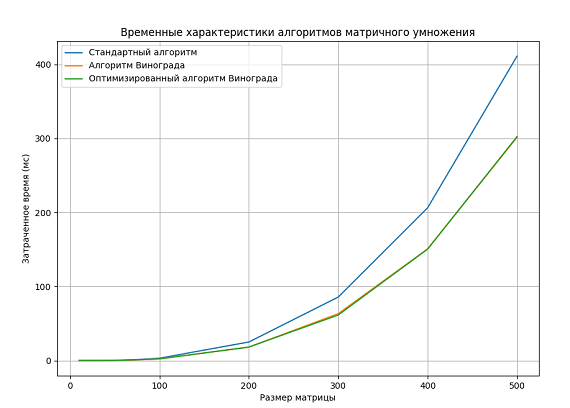
\includegraphics[trim=0 0 0 -5cm bb=0 0 570 650]{src/Graph}}
	\captionof{figure}{Процессорное время вычислений: четная размерность}
	\label{img:graph_sorted}
\end{center}
\newpage

\begin{center}
	\centering{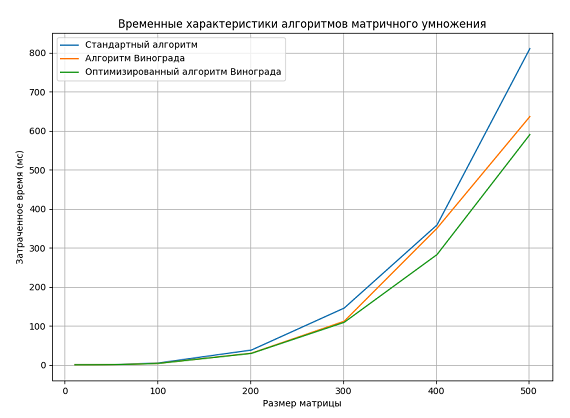
\includegraphics[trim=0 0 0 -5cm bb=0 0 570 650]{src/Graph1}}
	\captionof{figure}{Процессорное время вычислений: нечетная размерность}
	\label{img:graph_sorted1}
\end{center}
\newpage


\section*{Вывод}
\addcontentsline{toc}{section}{Вывод}


Теоретические результаты замеров и полученные практически результаты совпадают. Алгоритмы Винограда выполняются быстрее чем стандартный алгорим умножения мматриц примерно в $1.3$ раза.  Разница между алгоритмами становится более разлечима при увеличении размерности матриц.